% 菱形几何题配图（复现老板示例）：ABCD 菱形, ∠ABC=110°, E 在 BC 上,
% AE=EF, ∠AEF=110°, 连 CF 求 ∠DCF。
% 这份代码即"AI 生成层"的目标产物形态：LLM 只需产出这样的 TikZ 源码，
% 坐标全部由约束推导（\pgfmath），不允许手填像素位置，保证图形几何正确。
% 注意: TikZ 的 angle pic 从第一条边逆时针扫到第二条边，顶点顺序写反会画出优角。
\documentclass[border=10pt]{standalone}
\usepackage{tikz}
\usetikzlibrary{calc,angles,quotes,decorations.markings}

\begin{document}
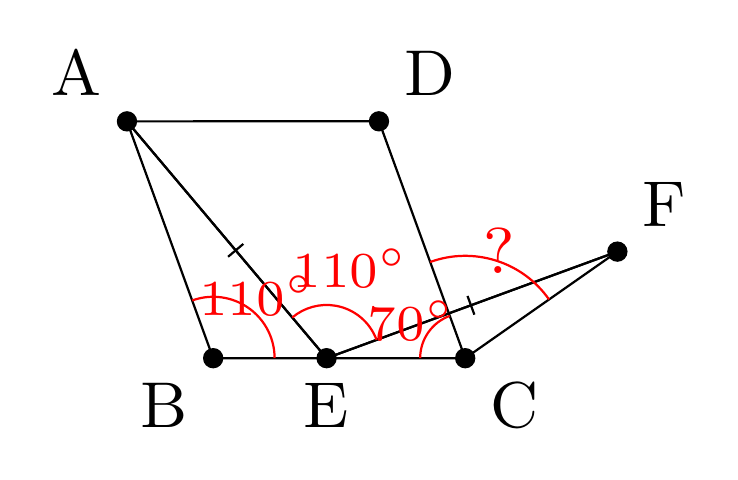
\begin{tikzpicture}[scale=3.2, every node/.style={scale=2.6, font=\small}]
  % --- 约束建点：边长 1，∠ABC=110° ---
  \coordinate (B) at (0,0);
  \coordinate (C) at (1,0);
  \coordinate (A) at ({cos(110)},{sin(110)});
  \coordinate (D) at ($(A)+(1,0)$);          % 菱形: AD ∥ BC 且等长
  \coordinate (E) at (0.45,0);               % E 在 BC 上（比例可参数化）
  % F: 将 A 绕 E 顺时针转 110°（保证 EA=EF 且 ∠AEF=110°）
  \pgfmathsetmacro{\fx}{0.45+(cos(110)-0.45)*cos(-110)-sin(110)*sin(-110)}
  \pgfmathsetmacro{\fy}{(cos(110)-0.45)*sin(-110)+sin(110)*cos(-110)}
  \coordinate (F) at (\fx,\fy);

  % --- 线段 ---
  \draw[thick] (A) -- (B) -- (C) -- (D) -- cycle;
  \draw[thick] (A) -- (E) -- (F);
  \draw[thick] (C) -- (F);

  % --- AE=EF 等长刻度 ---
  \draw[thick, decoration={markings, mark=at position 0.55 with {\arrow{|}}},
        postaction={decorate}] (A) -- (E);
  \draw[thick, decoration={markings, mark=at position 0.5 with {\arrow{|}}},
        postaction={decorate}] (E) -- (F);

  % --- 红色角标（弧内角方向：第二边相对第一边逆时针为正）---
  \pic[draw=red, thick, angle radius=3mm, angle eccentricity=1.25,
       "$110^\circ$" {text=red, font=\scriptsize}] {angle=C--B--A};
  \pic[draw=red, thick, angle radius=2.6mm, angle eccentricity=1.75,
       "$110^\circ$" {text=red, font=\scriptsize}] {angle=F--E--A};
  \pic[draw=red, thick, angle radius=2.2mm, angle eccentricity=1.45,
       "$70^\circ$" {text=red, font=\scriptsize}] {angle=D--C--E};
  \pic[draw=red, thick, angle radius=5mm, angle eccentricity=1.1,
       "?" {text=red, font=\small}] {angle=F--C--D};

  % --- 顶点与字母 ---
  \foreach \p/\l/\pos in {A/A/above left, B/B/below left, C/C/below right,
                          D/D/above right, E/E/below, F/F/above right} {
    \node[fill, circle, inner sep=1pt] at (\p) {};
    \node[\pos] at (\p) {\l};
  }
\end{tikzpicture}
\end{document}
